%%%%%%%%%%%%%%%%%%%%%%%%%%%%%%%%%%%%%%%%%
% baposter Landscape Poster
% LaTeX Template
% Version 1.0 (11/06/13)
%
% baposter Class Created by:
% Brian Amberg (baposter@brian-amberg.de)
%
% This template has been downloaded from:
% http://www.LaTeXTemplates.com
%
% License:
% CC BY-NC-SA 3.0 (http://creativecommons.org/licenses/by-nc-sa/3.0/)
%
%%%%%%%%%%%%%%%%%%%%%%%%%%%%%%%%%%%%%%%%%

%----------------------------------------------------------------------------------------
%	PACKAGES AND OTHER DOCUMENT CONFIGURATIONS
%----------------------------------------------------------------------------------------

\documentclass[landscape,a0paper,fontscale=0.285]{baposter} % Adjust the font scale/size here

\usepackage{lipsum}
\graphicspath{{images/}{../images/}}

\usepackage{menukeys} % for \keys
\usepackage{pifont}

\usepackage[utf8]{inputenc} 
\usepackage{graphicx} % Required for including images
\graphicspath{{figures/}} % Directory in which figures are stored

\usepackage[squaren, Gray, cdot]{SIunits}

\usepackage{amsmath} % For typesetting math
\usepackage{amssymb} % Adds new symbols to be used in math mode

\usepackage{booktabs} % Top and bottom rules for tables
\usepackage{enumitem} % Used to reduce itemize/enumerate spacing
\usepackage{palatino} % Use the Palatino font
\usepackage[font=small,labelfont=bf]{caption} % Required for specifying captions to tables and figures

\usepackage{multicol} % Required for multiple columns
\setlength{\columnsep}{1.5em} % Slightly increase the space between columns
\setlength{\columnseprule}{0mm} % No horizontal rule between columns

\usepackage{tikz} % Required for flow chart
\usetikzlibrary{shapes,arrows} % Tikz libraries required for the flow chart in the template

\newcommand{\compresslist}{ % Define a command to reduce spacing within itemize/enumerate environments, this is used right after \begin{itemize} or \begin{enumerate}
\setlength{\itemsep}{1pt}
\setlength{\parskip}{0pt}
\setlength{\parsep}{0pt}
}

\definecolor{lightblue}{rgb}{0.145,0.6666,1} % Defines the color used for content box headers




\begin{document}

\begin{poster}
{
headerborder=closed, % Adds a border around the header of content boxes
colspacing=1em, % Column spacing
bgColorOne=white, % Background color for the gradient on the left side of the poster
bgColorTwo=white, % Background color for the gradient on the right side of the poster
borderColor=lightblue, % Border color
headerColorOne=black, % Background color for the header in the content boxes (left side)
headerColorTwo=lightblue, % Background color for the header in the content boxes (right side)
headerFontColor=white, % Text color for the header text in the content boxes
boxColorOne=white, % Background color of the content boxes
textborder=roundedleft, % Format of the border around content boxes, can be: none, bars, coils, triangles, rectangle, rounded, roundedsmall, roundedright or faded
eyecatcher=true, % Set to false for ignoring the left logo in the title and move the title left
headerheight=0.1\textheight, % Height of the header
headershape=roundedright, % Specify the rounded corner in the content box headers, can be: rectangle, small-rounded, roundedright, roundedleft or rounded
headerfont=\Large\bf\textsc, % Large, bold and sans serif font in the headers of content boxes
%textfont={\setlength{\parindent}{1.5em}}, % Uncomment for paragraph indentation
linewidth=1pt % Width of the border lines around content boxes
}
%----------------------------------------------------------------------------------------
%	TITLE SECTION 
%----------------------------------------------------------------------------------------
%
{
\includegraphics[height=4em]{UCL.jpg}} 
{\bf\textsc{PROJET 3 : Amoniac et le g\'enie des proc\'ed\'es}\vspace{0.5em}} 
{\textsc{\small Cédric de Bellefroid - Cyril Denos - David Dispas  - Cassian Libeer  - Timothée Malengreau - Arnaud Paquet - John de Wasseige}} 
{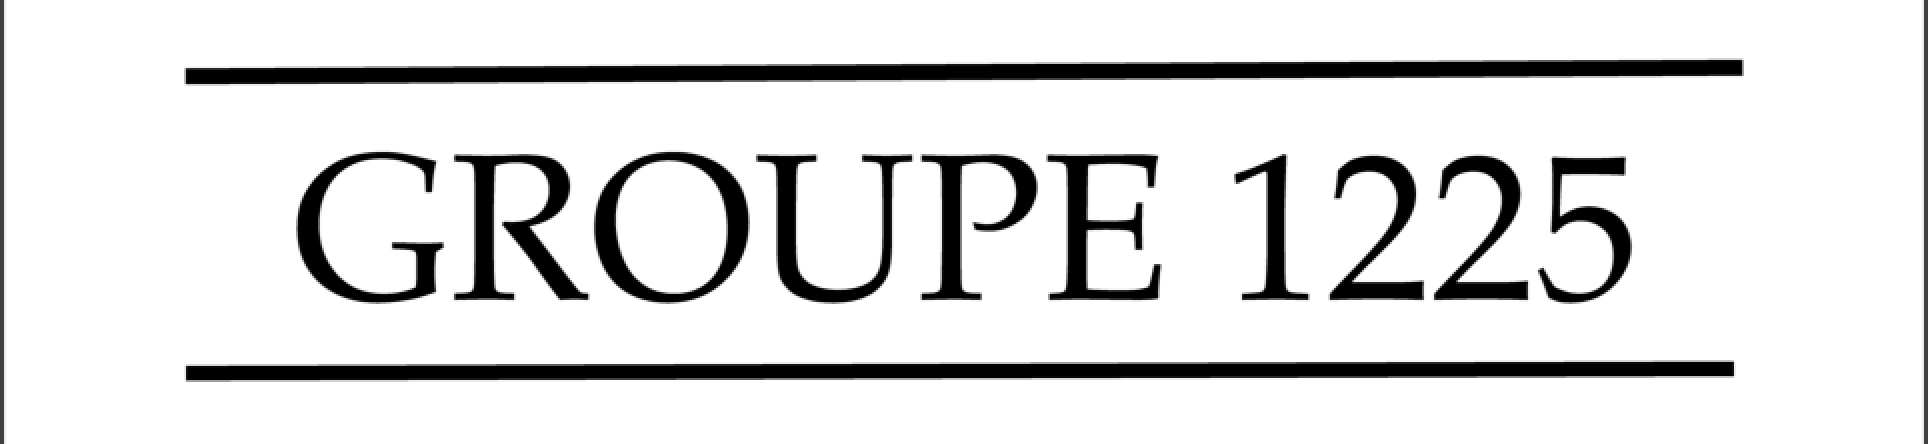
\includegraphics[height=4em]{groupe.png}} 

%----------------------------------------------------------------------------------------
%	BLOC 1 : RESUME
%----------------------------------------------------------------------------------------


%\background{
   %   \begin{tikzpicture}[remember picture,overlay]%
      %\draw (current page.north west)+(-2em,2em) node[anchor=north west]
      %{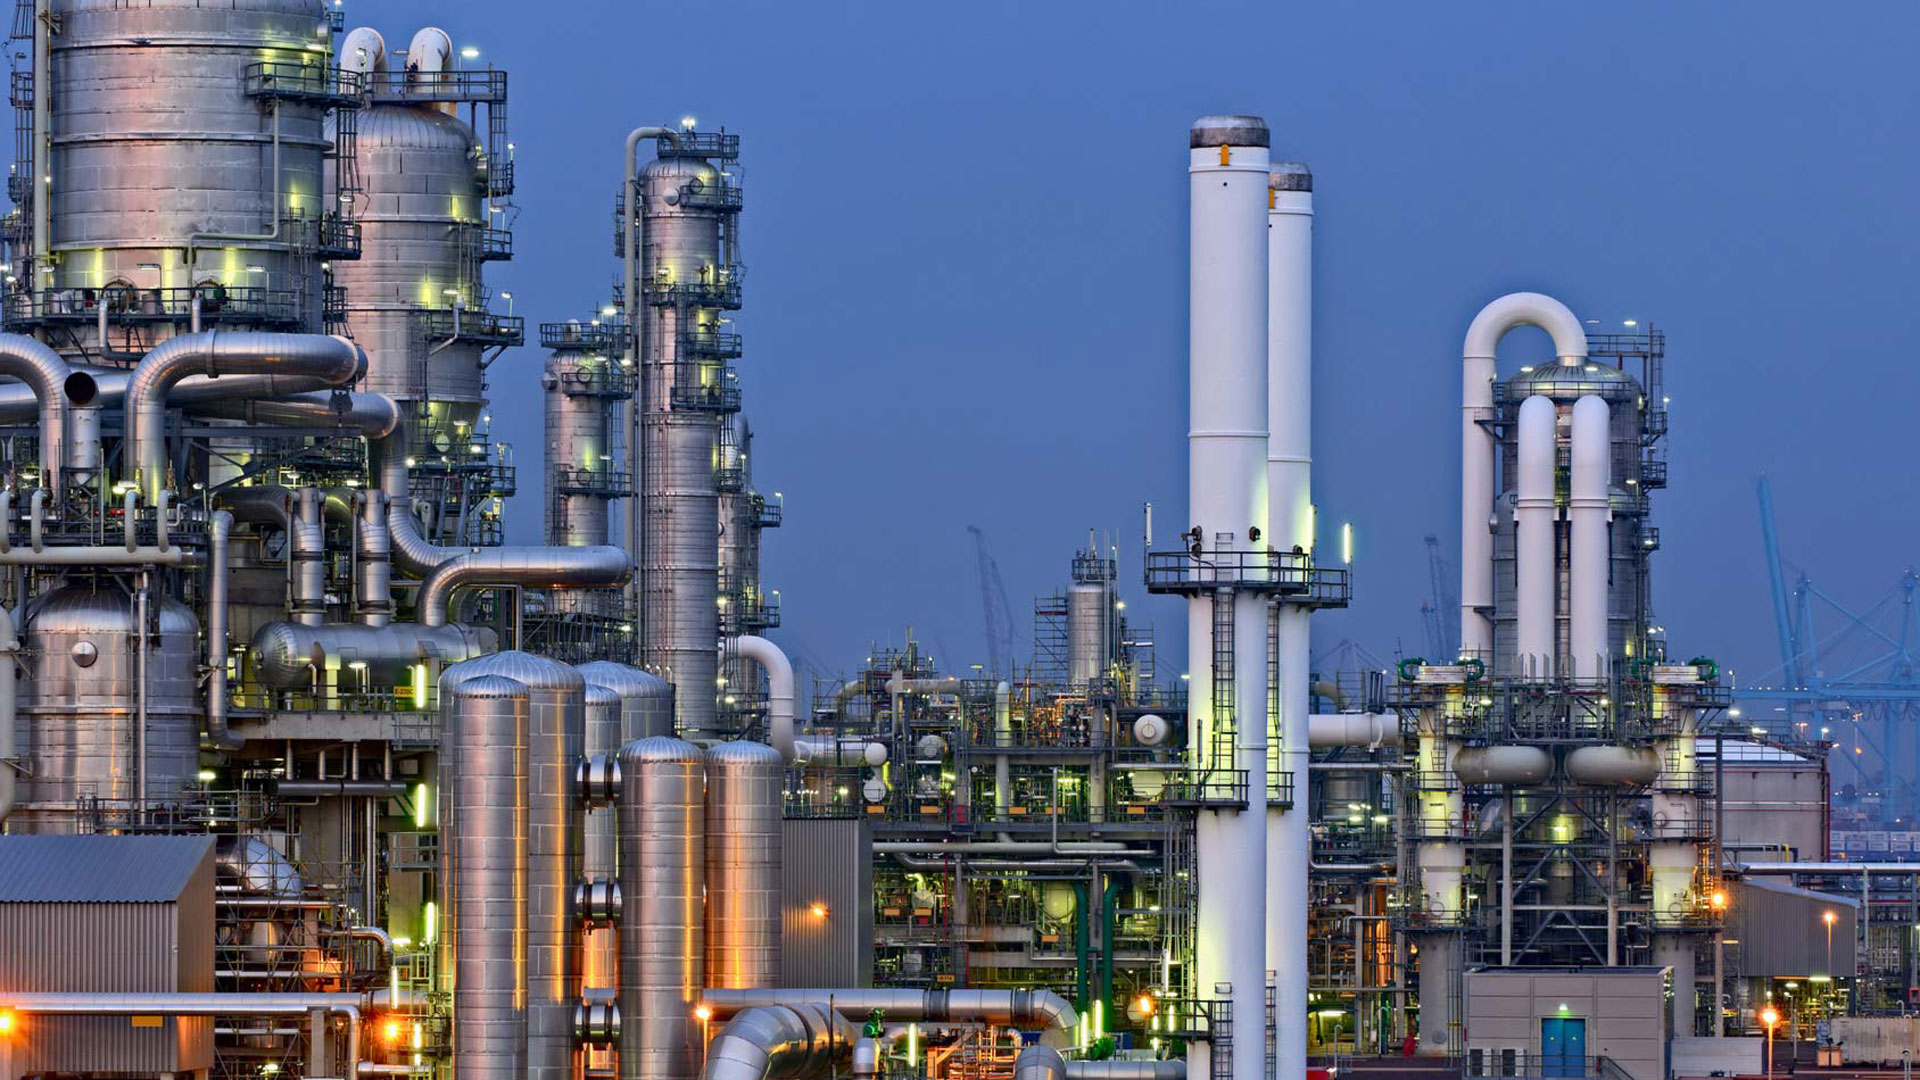
\includegraphics[height=2\textheight]{photousine}};
      %\end{tikzpicture}%
      %}
      
      
\headerbox{Résumé}{name=resume,column=0,row=0}{

% tkiz ball item
\newcommand*\circled[1]{\tikz[baseline=(char.base)]{
            \node[circle,ball color=purple, shade, 
 color=white,inner sep=1.2pt] (char) {\tiny #1};}}

% tkiz rounded item
\newcommand*\rounded[1]{\tikz[baseline=(char.base)]{
            \node[draw=none,ball color=purple, shade, 
 color=white, rounded corners=3.5pt, inner sep=2.5pt] (char) {\scriptsize #1};}}
 
 \textbf{			Etapes du projet}
 
  \begin{enumerate}

\item[\circled{\Large 1}] Compréhension du problème\\
\item[\circled{\Large 2}] Flow-sheet simplifié et bilan de matière\newline  \textbf{ Tâche 1}\\
\item[\circled{\Large 3}] Modélisation de la synthèse d'ammoniac avec Aspen+\newline \textbf{ Tâche 2}\\
\item[\circled{\Large 4}] Mini-HAZOP et soupape\newline \textbf{ Tâche 4} et \textbf{ Tâche 5}\\
\item[\circled{\Large 5}] Visites et ateliers\\
\item[\circled{\Large 6}] Etude environementale et améliorations \newline \textbf{ Tâche 3} et \textbf{ Tâche 8}\\
\item[\circled{\Large 7}] Synthèse, rapport final et présentation

 
  
    \end{enumerate}


%La première étape fut de comprendre le procédé chimique de la formation de l'amoniac. La réalisation  d'un flow sheet simplifié (\textbf{Tâche 2}) expliquant les différentes réactions a permis le calcul du bilan de matière du procédé complet (\textbf{Tâche 1})\\
%La production d'amoniac à grande échelle demande de grossed infrastructures. Qui dit grosses infrastructures dit systèmes de sécurités optimales et impact environementale.\\
%Ces sujets ont été développés au cours de ce projet, les \textbf{tâches 4} et\textbf{ 5} ont été consacrés au calcul du dimensionement d'une soupape de sécurité et d'un mini HAZOP.\\
%Les \textbf{tâches 3} porte sur une étude des différents gaz participants à l'effet de serre. La \textbf{tâche 8} est elle consacrée aux améliorations possible pour une telle infrastructure afin de limiter l'impact environementale.

}

%----------------------------------------------------------------------------------------
% BLOC 2 : TACHE 1
%----------------------------------------------------------------------------------------

\headerbox{Tâche 1}{name=tache1,column=1,row=0}{


\textbf{ Procédé Haber-Bosch - Flow-sheet simplifié}\\


\vspace{1em}
\begin{center}
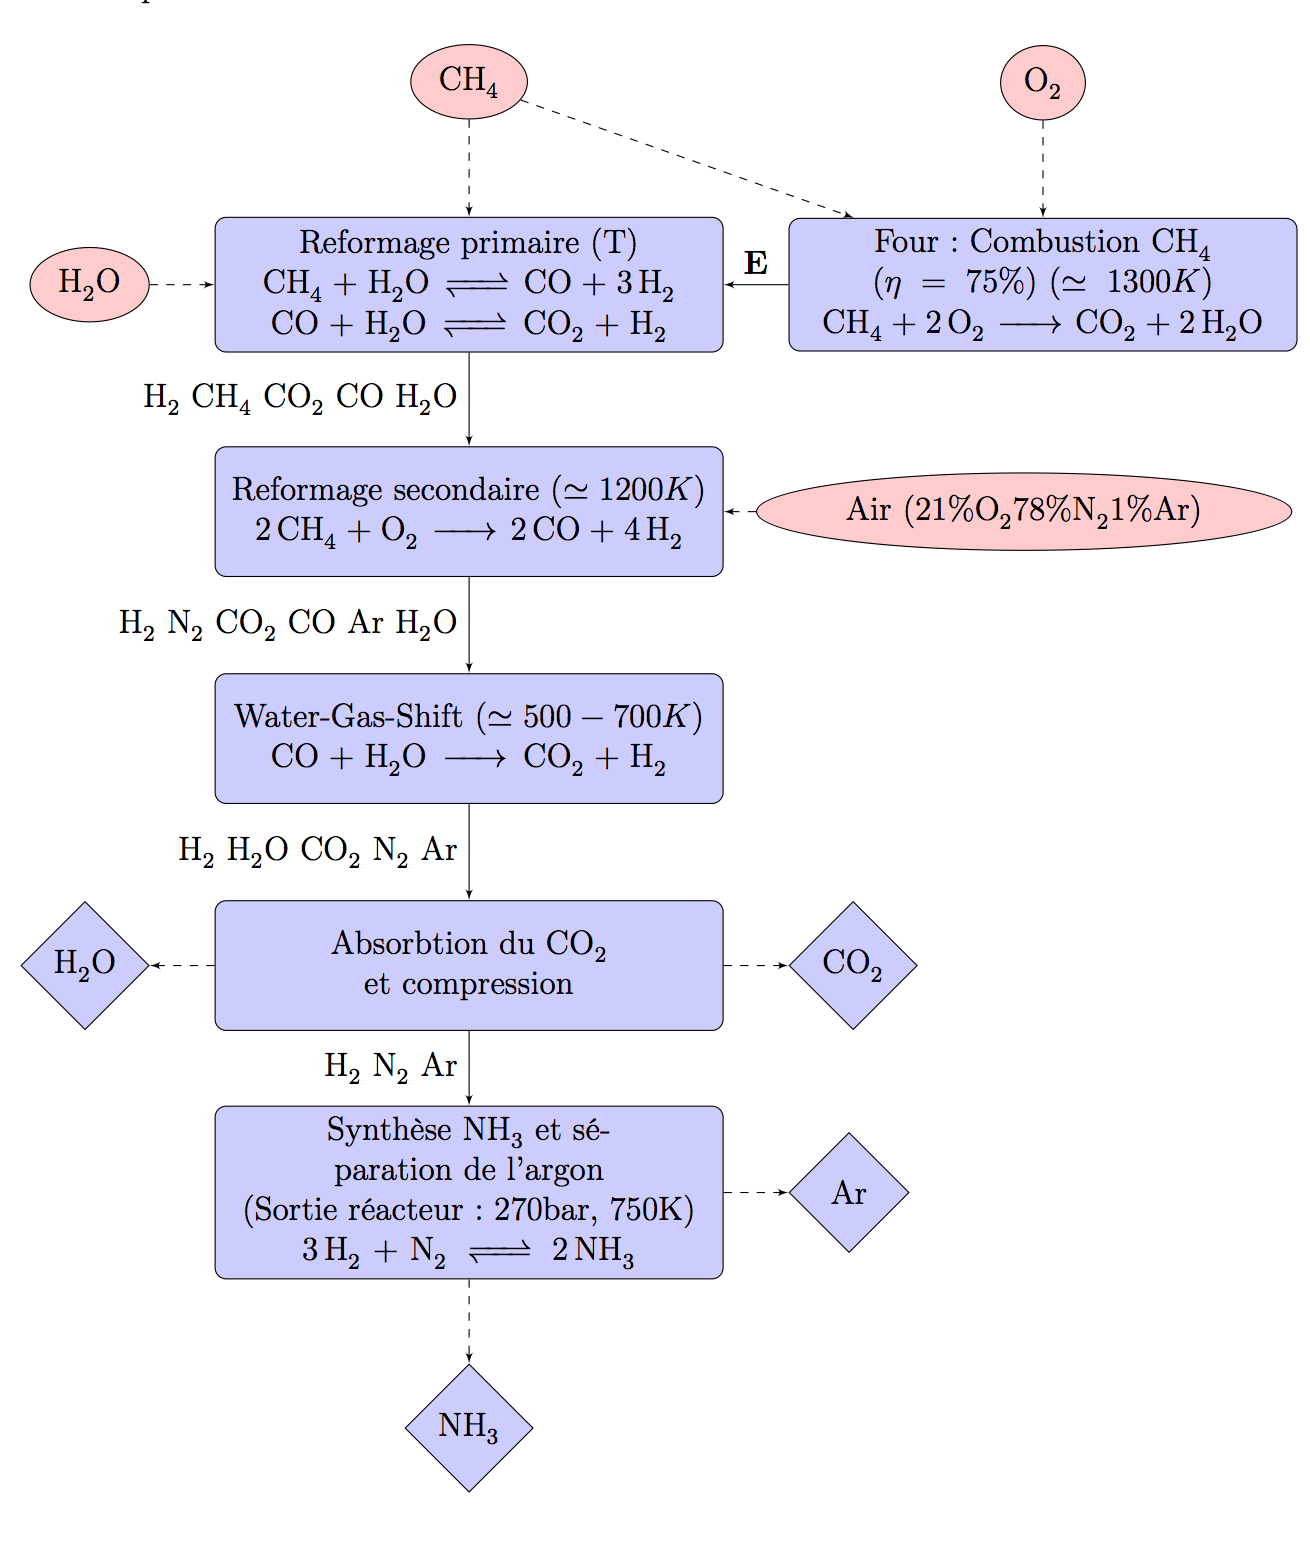
\includegraphics[width=1\linewidth]{PROC}
\end{center}

}



%----------------------------------------------------------------------------------------
%	BLOC 3 : TACHE 4 +5 
%----------------------------------------------------------------------------------------

\headerbox{Tâche 4 + 5}{name=tache45,column=2,span=2,row=0}{
\begin{multicols}{2}

\textbf{Dimmensionnement d'une soupape de sécurité}\\

\underline {Sans Isolation}\\

Pression normale de stockage : $7.8 barg$ à $20\ensuremath{^\circ}C$ \\

Pression maximale de tarage : $18.15barg$\\

Pression durant la décharge : $19$ $bar$. \\

\textbf{Section soupape} = $730mm^{2}$ \\
 
\underline{Avec isolation}\\

Coefficient d'échange avec l'extérieur :  $10\frac{W}{m^{2}K}$ et facteur environementale passe de $1$ à $0.15$\\

\textbf{Section soupape} = $110mm^{2}$. \\
\\
\\



\textbf{Mini-HAZOP}

\underline{Scénarios}
\begin{itemize}
\item Fuite de gaz
\item Problème réacteur
\item Blackout
\item ...
\end{itemize}

\underline{Conséquences}

\begin{itemize}
\item Incendie
\item Fuite
\item Explosion
\item ...
\end{itemize}

\underline{Mise en place de systèmes de sécurité} : \\
Soupapes, disques de ruptures, ...


%\begin{itemize}
%\item Soupape de sécurité
%\item Disque de rupture
%\item ...
%\end{itemize}


%Plusieurs scénarios catastrophoques ont été imaginés dans le mini-HAZOP; une fuite de gaz, problème dans un réacteur à réaction exomthermique, coupure de courant. Plusieurs possiblités sont parfois possibles pour éviter tout sur accident, il s'agit bien souvent de controler le gaz en jeu, ou la chaleur produite par certaines réactions et donc la surpression. Des soupapes de sécurité sont alors ajoutés la ou nécaissaire. La difficulté réside dans le dimmensionnement de ces appareils. En effet placer un dispositif trop petit ou avec une pression de tarage trop faible présente un danger, mais l'inverse peut l'etre aussi. D'ou l'importance de connaitre tous les facteurs qui interviennent dans le calcul du dimmensionnement des soupapes.\newline
%Ces calculs font intervenir des paramètres tel que la pression, la température, le type de gaz, le type de réservoir etc. Avec les données de l'énnoncé voici les résultats :\\
%La pression maximale de tarage de la soupape de sécurité vaut 
%\[ 105\% \cdot p_{\text{design}} = 16.8bar = 15.79barg \]
%La pression durant la décharge sera de $20.071 barg$. Cette pression est fort élevée car nous considérons ici le cas de feu. 
%La température du gaz durant la décharge sera de $50{\celsius}$. 


\end{multicols}
}



%----------------------------------------------------------------------------------------
% BLOC 4 : TACHE 3 + 8
%----------------------------------------------------------------------------------------

\headerbox{Tâche 3 + 8}{name=tache38,column=2,span=2,row=0,below=tache45}{

\begin{multicols}{2}
\vspace{1em}


Calculs réalisés pour une production de 1500 $Tonnes/Jour$  de $NH_{3}$ à $1000$ $K$)\\

\textbf{Emissions}\\

$CO_{2}$ : $1950$  $Tonnes/Jour$ \\

$T\ensuremath{^\circ} _{\text{réf1}} \searrow$   :   $CO_{2}\searrow$\\
\\
$H_{2}O$   :   $1940$ $Tonnes/Jour$\\

$H_{2}O\searrow$   :   $T\ensuremath{^\circ} _{\text{réf1}} \nearrow$\\
\\
\textbf{Fuites Potentielles}\\
$CH_{4}$ :
Impact =  $25$ x $CO_{2}$\\

$NH_{3}$ : Impact environnemental + Santé   \\

$Ar$ : Santé \\


\textbf{Améliorations}\\

Diminution des émissions de $CO_{2}$ $\rightarrow $ éléctrolyse 

\[ H_{2}O(g) \leftrightarrow \frac{1}{2}  O_{2}(g) + H_{2}(g) \]


\end{multicols}
\begin{center}
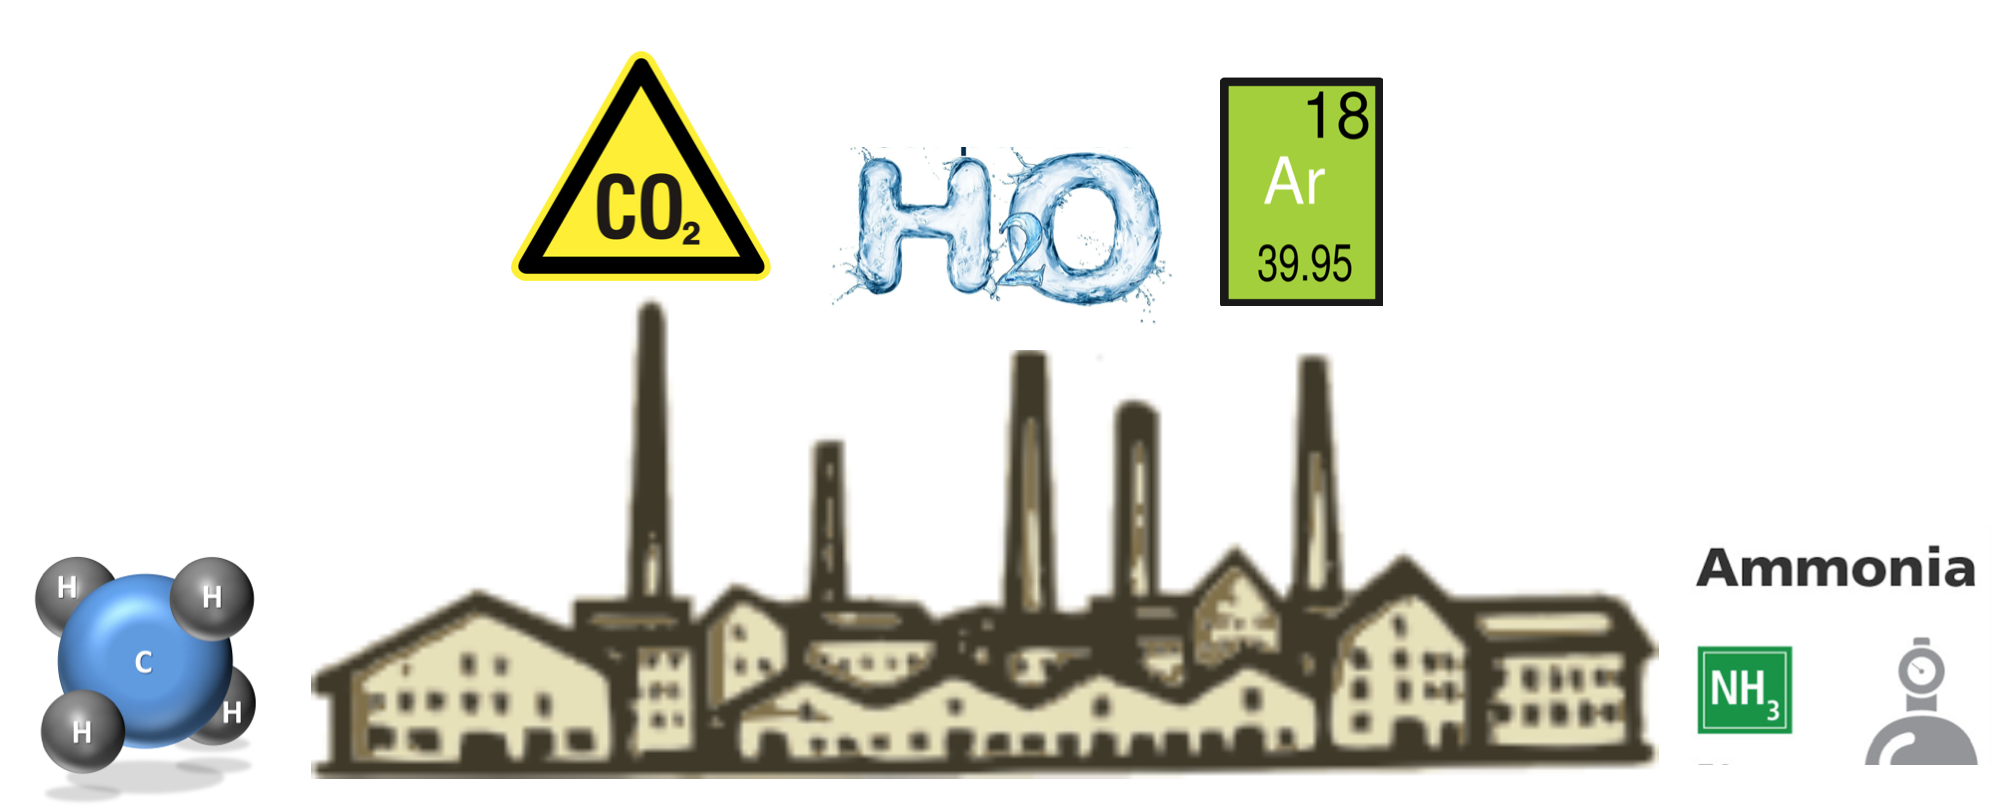
\includegraphics[width=0.6\linewidth]{usine}
\end{center}

}

%----------------------------------------------------------------------------------------
%	BLOC 5 : TACHE 2
%----------------------------------------------------------------------------------------

\headerbox{Tâche 2}{name=tache2,column=0,span=2,below=tache1}{ % This block's bottom aligns with the bottom of the conclusion block

\textbf{Etape de synthèse de l'ammoniac détaillée (Aspen Plus)}\\


\begin{center}
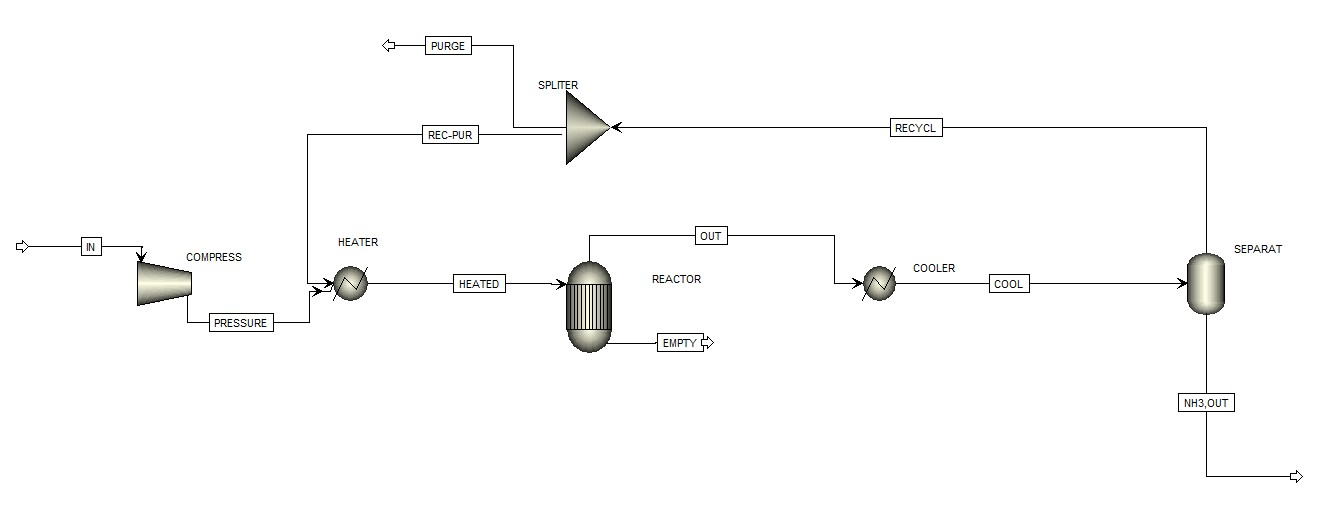
\includegraphics[width=1\linewidth]{flowsheet}
\end{center}



}


%%EXEMPLE TABLEAU

%%\begin{center}
%%\begin{tabular}{l l l}
%%\toprule
%%\textbf{Treatments} & \textbf{Response 1} & \textbf{Response 2}\\
%%\midrule
%%Treatment 1 & 0.0003262 & 0.562 \\
%%Treatment 2 & 0.0015681 & 0.910 \\
%%Treatment 3 & 0.0009271 & 0.296 \\
%%\bottomrule
%%\end{tabular}
%%\captionof{table}{Table caption}
%%\end{center}

%----------------------------------------------------------------------------------------

\end{poster}

\end{document}